\documentclass[11pt,]{book}
\usepackage{lmodern}
\usepackage{amssymb,amsmath}
\usepackage{ifxetex,ifluatex}
\usepackage{fixltx2e} % provides \textsubscript
\ifnum 0\ifxetex 1\fi\ifluatex 1\fi=0 % if pdftex
  \usepackage[T1]{fontenc}
  \usepackage[utf8]{inputenc}
\else % if luatex or xelatex
  \ifxetex
    \usepackage{mathspec}
  \else
    \usepackage{fontspec}
  \fi
  \defaultfontfeatures{Ligatures=TeX,Scale=MatchLowercase}
    \setmainfont[]{Palatino}
    \setmonofont[Mapping=tex-ansi,Scale=0.8]{Source Code Pro}
\fi
% use upquote if available, for straight quotes in verbatim environments
\IfFileExists{upquote.sty}{\usepackage{upquote}}{}
% use microtype if available
\IfFileExists{microtype.sty}{%
\usepackage{microtype}
\UseMicrotypeSet[protrusion]{basicmath} % disable protrusion for tt fonts
}{}
\usepackage{hyperref}
\hypersetup{unicode=true,
            pdftitle={Investigación Social Abierta},
            pdfauthor={Juan Carlos Castillo},
            pdfborder={0 0 0},
            breaklinks=true}
\urlstyle{same}  % don't use monospace font for urls
\usepackage{natbib}
\bibliographystyle{apalike}
\usepackage{color}
\usepackage{fancyvrb}
\newcommand{\VerbBar}{|}
\newcommand{\VERB}{\Verb[commandchars=\\\{\}]}
\DefineVerbatimEnvironment{Highlighting}{Verbatim}{commandchars=\\\{\}}
% Add ',fontsize=\small' for more characters per line
\usepackage{framed}
\definecolor{shadecolor}{RGB}{248,248,248}
\newenvironment{Shaded}{\begin{snugshade}}{\end{snugshade}}
\newcommand{\AlertTok}[1]{\textcolor[rgb]{0.94,0.16,0.16}{#1}}
\newcommand{\AnnotationTok}[1]{\textcolor[rgb]{0.56,0.35,0.01}{\textbf{\textit{#1}}}}
\newcommand{\AttributeTok}[1]{\textcolor[rgb]{0.77,0.63,0.00}{#1}}
\newcommand{\BaseNTok}[1]{\textcolor[rgb]{0.00,0.00,0.81}{#1}}
\newcommand{\BuiltInTok}[1]{#1}
\newcommand{\CharTok}[1]{\textcolor[rgb]{0.31,0.60,0.02}{#1}}
\newcommand{\CommentTok}[1]{\textcolor[rgb]{0.56,0.35,0.01}{\textit{#1}}}
\newcommand{\CommentVarTok}[1]{\textcolor[rgb]{0.56,0.35,0.01}{\textbf{\textit{#1}}}}
\newcommand{\ConstantTok}[1]{\textcolor[rgb]{0.00,0.00,0.00}{#1}}
\newcommand{\ControlFlowTok}[1]{\textcolor[rgb]{0.13,0.29,0.53}{\textbf{#1}}}
\newcommand{\DataTypeTok}[1]{\textcolor[rgb]{0.13,0.29,0.53}{#1}}
\newcommand{\DecValTok}[1]{\textcolor[rgb]{0.00,0.00,0.81}{#1}}
\newcommand{\DocumentationTok}[1]{\textcolor[rgb]{0.56,0.35,0.01}{\textbf{\textit{#1}}}}
\newcommand{\ErrorTok}[1]{\textcolor[rgb]{0.64,0.00,0.00}{\textbf{#1}}}
\newcommand{\ExtensionTok}[1]{#1}
\newcommand{\FloatTok}[1]{\textcolor[rgb]{0.00,0.00,0.81}{#1}}
\newcommand{\FunctionTok}[1]{\textcolor[rgb]{0.00,0.00,0.00}{#1}}
\newcommand{\ImportTok}[1]{#1}
\newcommand{\InformationTok}[1]{\textcolor[rgb]{0.56,0.35,0.01}{\textbf{\textit{#1}}}}
\newcommand{\KeywordTok}[1]{\textcolor[rgb]{0.13,0.29,0.53}{\textbf{#1}}}
\newcommand{\NormalTok}[1]{#1}
\newcommand{\OperatorTok}[1]{\textcolor[rgb]{0.81,0.36,0.00}{\textbf{#1}}}
\newcommand{\OtherTok}[1]{\textcolor[rgb]{0.56,0.35,0.01}{#1}}
\newcommand{\PreprocessorTok}[1]{\textcolor[rgb]{0.56,0.35,0.01}{\textit{#1}}}
\newcommand{\RegionMarkerTok}[1]{#1}
\newcommand{\SpecialCharTok}[1]{\textcolor[rgb]{0.00,0.00,0.00}{#1}}
\newcommand{\SpecialStringTok}[1]{\textcolor[rgb]{0.31,0.60,0.02}{#1}}
\newcommand{\StringTok}[1]{\textcolor[rgb]{0.31,0.60,0.02}{#1}}
\newcommand{\VariableTok}[1]{\textcolor[rgb]{0.00,0.00,0.00}{#1}}
\newcommand{\VerbatimStringTok}[1]{\textcolor[rgb]{0.31,0.60,0.02}{#1}}
\newcommand{\WarningTok}[1]{\textcolor[rgb]{0.56,0.35,0.01}{\textbf{\textit{#1}}}}
\usepackage{longtable,booktabs}
\usepackage{graphicx,grffile}
\makeatletter
\def\maxwidth{\ifdim\Gin@nat@width>\linewidth\linewidth\else\Gin@nat@width\fi}
\def\maxheight{\ifdim\Gin@nat@height>\textheight\textheight\else\Gin@nat@height\fi}
\makeatother
% Scale images if necessary, so that they will not overflow the page
% margins by default, and it is still possible to overwrite the defaults
% using explicit options in \includegraphics[width, height, ...]{}
\setkeys{Gin}{width=\maxwidth,height=\maxheight,keepaspectratio}
\IfFileExists{parskip.sty}{%
\usepackage{parskip}
}{% else
\setlength{\parindent}{0pt}
\setlength{\parskip}{6pt plus 2pt minus 1pt}
}
\setlength{\emergencystretch}{3em}  % prevent overfull lines
\providecommand{\tightlist}{%
  \setlength{\itemsep}{0pt}\setlength{\parskip}{0pt}}
\setcounter{secnumdepth}{5}
% Redefines (sub)paragraphs to behave more like sections
\ifx\paragraph\undefined\else
\let\oldparagraph\paragraph
\renewcommand{\paragraph}[1]{\oldparagraph{#1}\mbox{}}
\fi
\ifx\subparagraph\undefined\else
\let\oldsubparagraph\subparagraph
\renewcommand{\subparagraph}[1]{\oldsubparagraph{#1}\mbox{}}
\fi

%%% Use protect on footnotes to avoid problems with footnotes in titles
\let\rmarkdownfootnote\footnote%
\def\footnote{\protect\rmarkdownfootnote}

%%% Change title format to be more compact
\usepackage{titling}

% Create subtitle command for use in maketitle
\providecommand{\subtitle}[1]{
  \posttitle{
    \begin{center}\large#1\end{center}
    }
}

\setlength{\droptitle}{-2em}

  \title{Investigación Social Abierta}
    \pretitle{\vspace{\droptitle}\centering\huge}
  \posttitle{\par}
  \subtitle{Herramientas para la reproducibilidad, colaboración y comunicación académica}
  \author{Juan Carlos Castillo}
    \preauthor{\centering\large\emph}
  \postauthor{\par}
      \predate{\centering\large\emph}
  \postdate{\par}
    \date{2019-12-05}

\usepackage{booktabs}
\usepackage{amsthm}
\makeatletter
\def\thm@space@setup{%
  \thm@preskip=8pt plus 2pt minus 4pt
  \thm@postskip=\thm@preskip
}
\makeatother

\begin{document}
\maketitle

{
\setcounter{tocdepth}{1}
\tableofcontents
}
\hypertarget{presentaciuxf3n}{%
\chapter*{Presentación}\label{presentaciuxf3n}}
\addcontentsline{toc}{chapter}{Presentación}

Este es un libro orientado a describir herramientas de investigación reproducible enfocado a un público del ámbito de las ciencias sociales. Está inspirado sin duda por la noción de ciencia abierta, pero consiste básicamente en una guía práctica de software de escritura, comunicación y colaboración. El argumento básico es que el hacer ciencia abierta pasa por la reproducibilidad de nuestras investigaciones, y esto nos lleva a privilegiar el trabajo en texto plano.

Capítulos a desarrollar:

I. Preparando la investigación
1- Prerregistros
2- Reportes registrados

\begin{enumerate}
\def\labelenumi{\Roman{enumi}.}
\setcounter{enumi}{1}
\tightlist
\item
  Desarrollando la investigación
  1- Reproducibilidad
\end{enumerate}

\begin{itemize}
\tightlist
\item
  Organización: carpetas y path relativos
\item
  Orden de código
\item
  Colaboración en Github: forks, pull requests, issues y projects
\item
  Citando plano: Bibtex \& Zotero
  2- Control de versiones
\end{itemize}

\begin{enumerate}
\def\labelenumi{\Roman{enumi}.}
\setcounter{enumi}{2}
\tightlist
\item
  Comunicar la investigación
\end{enumerate}

1- Documentos reproducibles
- Markdown / Rmarkdown
- Tejiendo escritura y análisis: Knitr
- Pandoc, plantillas y salidas
- Documentos con parámetros

3- Publicación de resultados
- Publicación web vía Rmarkdown, blogdown \& bookdown
- Preprints, Postprints \& Acceso Abierto
- Presentando: Xaringan
- Open Science Framework \& SocArxiv
- Repositorios (Dataverse)

Apéndice: Implementación de Flujo X en Atom

\hypertarget{introducciuxf3n}{%
\chapter*{Introducción}\label{introducciuxf3n}}
\addcontentsline{toc}{chapter}{Introducción}

¿Es la ciencia una actividad cerrada? El uso de la palabra \emph{abierta} junto a \emph{ciencia} tiene sin duda un sentido crítico hacia formas de hacer ciencia que se caracterizan por las restricciones y el cierre. Parte importante de esta crítica tiene que ver con el difícil acceso a los resultados de investigaciones científicas, por barreras tanto comunicacionales como también económicas. El concepto de ``barreras de pago'' (paywall), una de las principales críticas a la ciencia actual, justamente consiste en que se debe pagar para poder acceder al conocimiento que en gran parte ha sido financiado por fondos públicos. Cuando el acceso al conocimiento está mediado por el tamaño de la billetera, sin duda surgen una serie de cuestionamientos sobre si esta forma de hacer y divulgar ciencia es la correcta.

\ldots{}

Este libro tiene dos fuentes de inspiración principales. La primera es un artículo de Jake Bowers titulado ``Six steps for a better relationship with your future self'', y la segunda es el trabajo de Kieran Healey, en particular su libro de ``The Plain Person's Guide to Plain Text Social Science.'' \citep{Healy2018PlainPersonGuide}

Idea 2: Existen muchos libros, páginas y foros de análisis de datos; también existen manuales de escriura tipo ``como hacer una tesis'' o ``diseño de investigación social'', pero casi no hay guias que discutan y apoyen las deciciones que se toman en el proceso mismo de la investigación. ¿Dónde escribo? ¿Cómo analizo los datos? ¿Cuál es la mejor manera de colaborar? Estos procesos son cerrados, tal como académicos y académicas se encierran en sus oficinas a producir con maneras sui-generis y que cada uno va escogiendo según le acomoda. \ldots{}

Temas a abordar:

\begin{itemize}
\tightlist
\item
  Acceso
\item
  Reproducibilidad
\item
  Colaboración
\item
  Comunicación
\end{itemize}

\hypertarget{preparando-la-investigaciuxf3n}{%
\chapter{Preparando la investigación}\label{preparando-la-investigaciuxf3n}}

\hypertarget{prerregistros}{%
\section{Prerregistros}\label{prerregistros}}

\hypertarget{reportes-registrados}{%
\section{Reportes registrados}\label{reportes-registrados}}

\hypertarget{documentaciuxf3n-de-datos}{%
\section{Documentación de datos}\label{documentaciuxf3n-de-datos}}

\hypertarget{desarrollando-la-investigaciuxf3n}{%
\chapter{Desarrollando la investigación}\label{desarrollando-la-investigaciuxf3n}}

\hypertarget{reproducibilidad}{%
\section{Reproducibilidad}\label{reproducibilidad}}

\hypertarget{organizaciuxf3n-carpetas-y-path-relativos}{%
\subsection{Organización: carpetas y path relativos}\label{organizaciuxf3n-carpetas-y-path-relativos}}

\hypertarget{orden-de-cuxf3digo}{%
\subsection{Orden de código}\label{orden-de-cuxf3digo}}

\hypertarget{colaboraciuxf3n-en-github-forks-pull-requests-issues-y-projects}{%
\subsection{Colaboración en Github: forks, pull requests, issues y projects}\label{colaboraciuxf3n-en-github-forks-pull-requests-issues-y-projects}}

\hypertarget{citando-plano-bibtex-zotero}{%
\subsection{Citando plano: Bibtex \& Zotero}\label{citando-plano-bibtex-zotero}}

\emph{Objetivo}: facilitar la inclusión de citas y referencias bibliográficas en documentos escritos en texto plano (Markdown / Latex).

\hypertarget{bibtex-zotero-y-better-bibtex-bbt}{%
\subsubsection{Bibtex, Zotero y Better BibTex (BBT)}\label{bibtex-zotero-y-better-bibtex-bbt}}

La forma general como funciona la inclusión de referencias en texto plano (Latex/Markdown) es tenerlas almacenadas en formato Bibtex (archivos en extensión \emph{.bib}). Este formato almacena las referencias en base a ciertos campos donde se incluye la información correspondiente. Por ejemplo:

\begin{verbatim}
@article{sabbagh_dimension_2003,
  title = {The Dimension of Social Solidarity in Distributive Justice},
  volume = {42},
  timestamp = {2014-09-26T12:30:41Z},
  number = {2},
  urldate = {2014-09-26},
  journal = {Social science information},
  author = {Sabbagh, Clara},
  year = {2003},
  pages = {255--276},
  file = {Snapshot:/storage/V5R7I29W/255.html:text/html},
  groups = {social justice theory,social justice theory}
}
\end{verbatim}

Luego, en la primera línea aparece la ``clave'' (key) de la referencia (en este caso sabbagh\_dimension\_2003), que permite llamarla en el texto como veremos más adelante.

Por supuesto, almacenar manualmente referencias en este formato bib no es muy amigable. Si bien una serie de softwares de administración de referencias tienen la opción de convertir fácilmente la colección o parte de ella a formato .bib, el problema es que si se añade una referencia en el software, cada vez habría que convertir/sincronizar nuevamente a .bib para mantener esta base también actualizada. Por lo tanto, lo ideal sería que una colección .bib se actualizara automáticamente desde un software de gestión de referencias. La solución que por ahora se recomienda es usar la aplicación Better(bib)tex (BBT), que funciona dentro de Zotero (www.zotero.org). Ambos gratuitos y de código abierto, así que ok. BBT genera una colección .bib en base a librerías Zotero, se configura solo una vez y luego se mantiene sincronizada, para no preocuparse más del asunto.

\textbf{Zotero / BBT}: El funcionamiento de Zotero queda fuera del alcance de este tutorial, solo nos enfocaremos en el vínculo con BBT.

\begin{itemize}
\tightlist
\item
  Bajar Zotero 5 standalone \url{https://www.zotero.org/}
\item
  Bajar el archivo para instalar BBT, ultima actualización al 19 oct 2017: \url{https://github.com/retorquere/zotero-better-bibtex/releases/download/v5.0.28/zotero-better-bibtex-5.0.28.xpi}
\item
  En Zotero, Tools - Add-ons
\item
  En la ventana emergente, esquina superior derecha, menú con ícono de tuerca, Install Add-on from file, dar path hacia el archivo xpi de BBT
\item
  Reiniciar Zotero
\item
  Exportando / sincronizando con archivo Bib:

  \begin{itemize}
  \tightlist
  \item
    posicionarse sobre una carpeta de referencias de Zotero (que también puede ser la colección completa, o sea My Library), botón derecho, export collection, y en el formato escoger ``Better BibTex''.
  \item
    En las ``translator options'' marcar ``keep updated'', que sincroniza el bib en cuanto se agrega una referencia a Zotero

    \begin{itemize}
    \tightlist
    \item
      Luego escoger directorio donde se graba (que puede ser el mismo de Zotero). Se recomienda que el nombre del archivo no lleve espacios.
    \end{itemize}
  \end{itemize}
\item
  Para revisar las opciones de la sincronización, ir a edit\textgreater{}preferences aparece una pestaña nueva al final a la derecha de BBT. En esa pestaña hay una serie de opciones que luego se pueden explorar, por lo pronto ir a la pestaña ``Automatic export'' donde debería aparecer en el listado la carpeta seleccionada para exportar. En ``automatic export'' seleccionar ``on change'', que hace que cada vez que se cambia algo en Zotero de esa carpeta, se cambia también en el archivo .bib exportado y sincronizado.
\item
  Más información sobre BBT: \url{https://github.com/retorquere/zotero-better-bibtex/wiki}
\item
  (NOTA: en caso que no funcione, puede ser por problemas exportando con la nueva versión de Zotero (5); la adaptación de BBT se encuentra en desarrollo, ver \url{https://github.com/retorquere/zotero-better-bibtex/issues/555}); por lo tanto, si hay problemas con la instalación tradicional con el Zotero 5, se recomienda instalar la versión 4 de Zotero Standalone, y bajar la versión previa correspondiente de la extensión \url{https://github.com/retorquere/zotero-better-bibtex/releases/tag/1.6.100})
\end{itemize}

\hypertarget{sobre-exportar-referencias-en-trabajo-colaborativo}{%
\paragraph{Sobre exportar referencias en trabajo colaborativo}\label{sobre-exportar-referencias-en-trabajo-colaborativo}}

\begin{itemize}
\tightlist
\item
  Aquí, una opción es dar el link desde Markdown/Latex al archivo completo de Zotero (del autor a cargo), pero en general es muy pesado y contiene todas las referencias, no el subgrupo que se utiliza en el paper. Por lo tanto, se recomienda hacer lo siguiente:

  \begin{itemize}
  \tightlist
  \item
    crear una colección/carpeta compartida de Zotero (asumiendo escenario de trabajo colaborativo) donde se copian las referencias que se utilizan en el paper. Esto es fácil en Zotero, solo se arrastran, y no hace que toda la información se duplique, es solo un link. Como es compartida, cualquier miembro del equipo puede modificar. Precaución: el nombre de esta carpeta sin espacios y sin acentos
  \item
    El coordinador/primer autor exporta esta colección a la carpeta del proyecto colaborativo (eventualmente un dropbox) donde está el tex/md. Para ello, botón derecho sobre la carpeta, ``export library'', seleccionar \emph{format Better Bibtex}, y nuevamente, muy importante: check box ``keep updated'', así cualquier cambio que se haga en la colección desde Zotero se reflejará en el .bib. Guardar en la carpeta donde se encuentra el archivo tex
  \item
    Luego, revisar en la pestaña de BBT de preferencias, en automatic export, que la carpeta efectivamente está en el listado. Además, marcar la opción ``on change''.
  \end{itemize}
\end{itemize}

\hypertarget{referenciando-en-tex}{%
\subsubsection{Referenciando en TEX}\label{referenciando-en-tex}}

\begin{itemize}
\tightlist
\item
  En el preámbulo (hay diferentes opciones de formato, pero para estilo clásico APA):
\end{itemize}

\begin{verbatim}
\usepackage{natbib} % for Bibtex
\bibliographystyle{apalike}
\end{verbatim}

\begin{itemize}
\tightlist
\item
  algunos estilos vienen por defecto, si no se pueden bajar en: \url{https://es.sharelatex.com/learn/Natbib_bibliography_styles}
\item
  si el estilo no está por defecto, guardar en la carpeta donde se encuentra el .bib
\item
  obligatorio: tiene que definirse un estilo para que funcione la compilación de la bibliografía (al menos esa fue mi experiencia)
\item
  Y luego, donde se quiera la bibliografía, (usualmente, alfinal, antes de end(document))
\end{itemize}

\begin{verbatim}
\bibliography{micoleccion}
\end{verbatim}

\begin{itemize}
\tightlist
\item
  aquí va el nombre de la colección, cuidado con no darle nombre con espacios, y tampoco terminarla con .bib
\item
  También se puede indicar con path relativos, ej:
\end{itemize}

\begin{verbatim}
 \bibliography{../../bib/micoleccion}
\end{verbatim}

\begin{itemize}
\item
  donde ``../'' es para subir un nivel en la estructura de directorios
\item
  Con esto, ya se puede comenzar a citar con las distintas opciones; ver \url{https://gking.harvard.edu/files/natnotes2.pdf}
\item
  Y también se puede creando un link simbólico en la carpeta respectiva que apunte hacia el archivo .bib de la carpeta Zotero, de esa manera no es necesario especificar la ruta.
\item
  Para mayores detalles referentes a natbib y en general bibliographic management en Latex ver \url{https://es.sharelatex.com/learn/Bibliography_management_with_natbib}

  \begin{itemize}
  \tightlist
  \item
    Algunos issues con Latex: si se añade alguna cita a la carpeta Zotero, si bien esto es actualizado automáticamente en el bib, no necesariamente es reconocido al momento de citar. Por eso, se recomienda tener abierto el archivo .bib en el editor de tex en otra pestaña, y si la referencia no aparece al intentar citar compilar el bib, esto hace que queden disponibles para citar (lo que se ve en el .bbl, donde se encuentran las referencias citadas en el texto)

    \begin{itemize}
    \tightlist
    \item
      Por lo visto, las referencias en el .bbl se van sumando, y no se borran. Por lo tanto, puede pasar que se cite algo en alguna ocasión, pero si esa cita se decide borrar va a seguir de todas maneras apareciendo en la bibliografía final. Para ajustar esto, cuando se genere una versión más definitiva del documento, borrar el bbl y compilar el tex nuevamente.
    \item
      Atención: si se quiere cambiar el estilo (

      \bibliographystyle{}

      ), a veces no lo reconoce y se queda con el anterior o arroja error; la opción que me resulta es borrar los archivos aux y bbl, y luego compilar nuevamente.
    \item
      También hay problemas cuando alguna entrada del archivo .bib no tiene el año, en este archivo aparecen como ???? y esto crea dificultades de compilación. Importante: arreglar esto en Zotero (no en bib ni bbl), sincronizar nuevamente y compilar.
    \end{itemize}
  \end{itemize}
\end{itemize}

\hypertarget{referenciando-en-markdown}{%
\subsubsection{Referenciando en Markdown}\label{referenciando-en-markdown}}

\begin{itemize}
\item
  se establece la ruta al archivo bib en el YAML header, al comienzo del documento, por ejemplo:

\begin{verbatim}
---
bibliography:
- 'MyLibrary.bib'
---
\end{verbatim}

  \begin{itemize}
  \tightlist
  \item
    para citar, se debe escribir el ``citation key'' de la referencia correspondiente.
  \item
    la lista de referencias aparece automáticamente al final del documento
  \item
    el estilo de bibliografía se debe indicar adicionalmente, basado en un archivo .csl correspondiente.Un listado de estilos disponibles se encuentra en: \url{https://www.zotero.org/styles}
  \item
    Luego el csl se agrega al YAML. Ej:
  \end{itemize}

\begin{verbatim}
---
bibliography:
- MyLibrary.bib
- csl: apa.csl
---
\end{verbatim}

  \begin{itemize}
  \item
    Alternativas para automatizar la inserción de referencias: ya que insertar referencias manualmente es muy engorroso, hay algunas alternativas de automatización que generan un flujo de trabajo similar al de insertar citas y bibliografía en Word/Open Office vía Zotero. El mejor entorno que conozco para hacer esto es Atom, porque sirve tanto para Latex como para Markdown. También hay una forma en Rstudio vía la librería/add-in ``citr''. Comenzamos con esta:
  \item
    Usando Rstudio - citr \url{https://github.com/crsh/citr}:

    \begin{itemize}
    \tightlist
    \item
      Al instalar Rmarkdown, se instala automaticamente pandoc al interior de la carpeta de Rstudio (/usr/lib/rstudio/bin/pandoc), donde están los ejecutables pandoc y pandoc-citeproc. Por lo tanto, en archivos Rmd basta dar el nombre del archivo/path al bib en el YAML header para que encuentre la bibliografía y la compile correctamente.
    \item
      Instalar citr
    \item
      reiniciar
    \item
      Luego en el add-in (desplegable, o tools/add-ins) aparece ``insert citations'', si está bien especificado el bib en el YAML debería aparecer aquí la lista de referencias.
    \end{itemize}
  \end{itemize}
\end{itemize}

\hypertarget{markdown-xaringan}{%
\subsubsection{Markdown / Xaringan}\label{markdown-xaringan}}

\begin{verbatim}
[Xaringan]() es una librería de R que permite generar presentaciones en html basadas en [remark](https://remarkjs.com), que utiliza una estructura simple de markdown. Básicamente, lo que hace Remark es compilar un markdown + un poco de css a un html, y Xaringan se encarga de la parte css así que el usuario trabaja (casi) solo en markdown.

El problema: para generar el html no pasa por pandoc, así que no sigue la misma lógica de las citas de markdown. Pero ... todo tiene una vuelta de tuerca, y en este caso se puede utilizando el paquete de R [RefManageR](https://github.com/ropensci/RefManageR).

1. Indicar paquete y librería: en un chunk de setup luego del YAML header. La librería se indica con la función ReadBib de RefManageR (en este caso, en el mismo directorio, si no dar el path)


````
  ```{r setup, include=FALSE}
   options(htmltools.dir.version = TRUE)
   pacman::p_load(RefManageR)
   bib <- ReadBib("merit_pref_int.bib", check = FALSE)
  ```
````


2. Para citar: los comandos básicos del RefManageR son Cite(), Citep() y Citet() (como en natbib), y en el paréntesis va el nombre del objeto generado antes y que contiene las referencias (bib) y la clave de la referencia como está en el Bibtex. Ejemplo: Cite(bib, "castillo_2018"). Ahora, como se trata de compilar a html sin pasar por pandoc, hay que dar la instrucción para que R/RefManageR hagan el trabajo, así que la cita se escribe en un mini-chunk de código:  r Cite (bib, "castillo_2018")

3. Algunas complicaciones del RefManagerR

  - muy estricto con la librería .bib, si hay algo que falta en algún campo va a reportar el error. Por lo tanto, a menos que el .bib de la colección completa esté perfecto, es mejor hacer una subcolección de Zotero con las referencias y esta exportarla como Bibtext a la carpeta correspondiente donde se está trabajando
  - se puede usar el Zotero Picker en Atom para facilitar el trabajo, pero hay que sacarle manualmente la @ inicial que es automática para referencias en markdown que pasan por pandoc

4. Para generar las referencias: en la lámina que corresponde, incluir:

````
```{r, results='asis', echo=FALSE}
PrintBibliography(bib)
```
````

## Usando Atom para flujo de trabajo académico en texto plano con citas

Aquí hay tres cosas que ver: insertar, preview y convert

  - Insertar:
      - para insertar citaciones lo más fácil es instalar el zotero-picker, que automáticamente detecta la librería bib que se encuentra en la misma carpeta de Zotero (vía Better Bibtex). Funciona igual que el plugin clásico para procesadores de texto, shortcut alt-z
      - otra alternativa que se puede instalar en paralelo es el autocomplete-bibtex, que busca la cita una vez escrito @ y las tres primeras letras, asumiendo que la bib está en el mismo directorio (o probar también si funciona dando el path con YAML)

  - Preview
      - markdown se puede visualizar simultáneamente en atom con el paquete markdown-preview-plus (MPP) (ctrl+shift+m). Para que aparezcan las citas y la bibliografía se deben hacer un par de ajustes (* si se instala Rmarkdown, pandoc ya está instalado, pero en el directorio de R y Atom no lo reconoce, por eso recomiendo instalarlo nuevamente):
        - instalar pandoc, en ubuntu
          - sudo apt-get update
          - sudo apt-get install pandoc
          - chequear instalado: dpkg -L pandoc
        - instalar pandoc citeproc
          - sudo apt-get update
          - sudo apt-get install pandoc-citeproc
        - en las opciones del paquete
          - enable pandoc parser
          - pandoc options: citations
        - en el documento .md crear al principio un YAML header con el path hacia el bib:

````
---
bibliography:
- '/media/ntfs/Dropbox/zoterojcydocs/MyLibrary.bib'
---
````

  - con esto, luego el MPP muestra las citas (en el preview)


  - Convertir: el paquete pandoc-convert (hasta ahora) no convierte las citas, solo el texto. Lo que funciona es vía linea de comando, abriendo terminal desde atom y:
\end{verbatim}

\begin{verbatim}
pandoc -s -S --bibliography MyLibrary.bib --filter pandoc-citeproc --csl apa-cv.csl inequality_perception_issp.md -o inequality_perception_issp.html
\end{verbatim}

\hypertarget{control-de-versiones}{%
\section{Control de versiones}\label{control-de-versiones}}

Pasos

\begin{enumerate}
\def\labelenumi{\arabic{enumi}.}
\tightlist
\item
  Instalar Git a nivel local
\end{enumerate}

sudo apt-get install git

\begin{enumerate}
\def\labelenumi{\arabic{enumi}.}
\setcounter{enumi}{1}
\item
  Abrir cuenta en Github
\item
  Vincular local con Github
\end{enumerate}

En terminal:

\begin{verbatim}
git config --global user.email "you@example.com"
git config --global user.name "Your Name"
\end{verbatim}

\hypertarget{comunicando-la-investigaciuxf3n}{%
\chapter{Comunicando la investigación}\label{comunicando-la-investigaciuxf3n}}

\hypertarget{documentos-reproducibles}{%
\section{Documentos reproducibles}\label{documentos-reproducibles}}

En la investigación académica en general el proceso de escritura se encuentra separado del análisis, en programas y documentos distintos. El traspaso de información entre el programa de análisis y el programa de edición de texto se realiza con un clásico: cortar y pegar.

\emph{¿Cuáles son las desventajas de cortar y pegar?}

\begin{itemize}
\item
  La principal es el límite a la reproducibilidad. ¿Cómo identificar los análisis que finalmente son reportados?
\item
  Eficiencia: cada vez que se realicen cambios en los análisis, nuevamente implica cortar-pegar, y es difícil llevar un registro apropiado de las versiones de los documentos.
\end{itemize}

Los \textbf{documentos dinámicos} permiten lidiar con las limitaciones anteriores, ya que los análisis y resultados están en un mismo documento. Esto es posible ya que se combinan dos lenguajes en texto plano: escritura y código de análisis. La clave es que el programa de edición y de análisis pueda identificar qué secciones del texto corresponden a escritura y cuáles corresponden a análisis.

\hypertarget{sobre-texto-plano}{%
\subsection{Sobre texto plano}\label{sobre-texto-plano}}

\emph{¿Por qué escribir en texto plano en lugar de un programa que me muestre inmediatamente el texto y su formato (tipo Word)?}
Hay múltiples razones, solo resalto dos:

1 - \textbf{Propiedad}: los contenidos guardados en formatos de procesadores comerciales (como Word) dependen del pago de una licencia para poder leerse. Si el software es imposible leerlos, por lo tanto la propiedad de los contenidos guardados en ese formato no son del autor/a, sino de la empresa de software. El texto plano no depende de un software comercial para poder leerse ni modificarse.

2 - \textbf{Flexibilidad en incorporación de texto y análisis}: el escribir en texto plano permite incluir en un mismo documento elementos de escritura y de análisis de datos realizado en texto plano, por lo tanto no se requiere cortar ni pegar en otro documento.

Actualmente existen una serie de herramientas que facilitan la elaboración de documentos dinámicos, en particular basados en la librería \texttt{knitr} (tejer). Esta librería permite generar documentos escritos en lenguaje Markdown y análisis realizado en R.

\hypertarget{markdown}{%
\subsection{Markdown}\label{markdown}}

Combinar texto y código de análisis requiere que ambos puedan ser generados en una misma plataforma. Y para poder hacer esto, una solución es que lo que se escriba en el documento sea libre de plataforma. El texto plano es una forma de escribir que no requiere ningún programa especial para poder acceder o generar un documento. El ejemplo más cercano para los usuarios de Windows son los archivos .txt, que se pueden abrir con cualquier editor simple.

Ahora bien, también para escribir necesitamos elementos de edición, como por ejemplo encabezados, listas, imágenes, negritas, cursivas. Y es aquí donde Markdown permite integrar elementos de edición en texto plano. ¿Cómo se hace? incorporando código o ``marcas'' de edición, pero de la manera más simple posible (de ahí el nombre markdown, marcas bajas o pocas marcas). Estas marcas indican las partes del texto que luego serán interpretadas de una manera especial al momento de convertir el documento a otro formato que sea más amigable a la publicación (como html o pdf). Por lo tanto, la manera de trabajar es en base a un editor de texto plano, y que al final se convierte a un documento publicable.

\hypertarget{marcas-de-ediciuxf3n}{%
\subsubsection{Marcas de edición}\label{marcas-de-ediciuxf3n}}

\textbf{Títulos}

Los títulos se generan mediante el caracter \# , de la siguiente manera:

\begin{verbatim}
# Titulo 1
## Título 2
### Título 3
\end{verbatim}

Lo que al convertir genera lo siguiente:

Titulo 1

Titulo 2

Titulo 3

\textbf{Negritas / cursivas}

\begin{verbatim}
esto es **negrita**
esto es *cursiva*
\end{verbatim}

esto es \textbf{negrita}
esto es \emph{cursiva}

\begin{center}\rule{0.5\linewidth}{\linethickness}\end{center}

\textbf{Listas}

\begin{verbatim}
    ```
    - item 1
    - item 2
      - item sub 2
        - item sub 2 sub 2

    1. item
    2. item
        - item
        - item
    ```
\end{verbatim}

\begin{itemize}
\tightlist
\item
  item 1
\item
  item 2

  \begin{itemize}
  \tightlist
  \item
    item sub 2

    \begin{itemize}
    \tightlist
    \item
      item sub 2 sub 2
    \end{itemize}
  \end{itemize}
\end{itemize}

\begin{enumerate}
\def\labelenumi{\arabic{enumi}.}
\tightlist
\item
  item
\item
  item

  \begin{itemize}
  \tightlist
  \item
    item
  \item
    item
  \end{itemize}
\end{enumerate}

\begin{center}\rule{0.5\linewidth}{\linethickness}\end{center}

\textbf{Web links}

\href{http://www.facso.uchile.cl/}{Facso}
\url{http://www.facso.uchile.cl/}

\begin{verbatim}
[Facso](http://www.facso.uchile.cl/)
[http://www.facso.uchile.cl/](http://www.facso.uchile.cl/)
\end{verbatim}

\begin{center}\rule{0.5\linewidth}{\linethickness}\end{center}

\textbf{Imágenes}

En general:

\begin{verbatim}
![](ruta-a-imagen/imagen.jpg)
\end{verbatim}

Ejemplo:

\begin{verbatim}
![](images/knitr.png)
\end{verbatim}


\includegraphics{images/knitr.png}

Esta imagen se encuentra en el subdirectorio images

Si se desea agregar otros elementos de edición como centrado o tamaño, hay que recurrir a marcas de html:

\begin{verbatim}
<p align="center">
  <img src="images/knitr.png" width="240px" height="280px"/>
</p>
\end{verbatim}

Como se puede ver, markdown está hecho para edición simple, y cualquier aspecto que requiera una mayor edición implica recurrir a otros lenguajes, en este caso html.

\textbf{Listas}

\begin{verbatim}
    ```
    - item 1
    - item 2
      - item sub 2
        - item sub 2 sub 2

    1. item
    2. item
        - item
        - item
    ```
\end{verbatim}

\begin{itemize}
\tightlist
\item
  item 1
\item
  item 2

  \begin{itemize}
  \tightlist
  \item
    item sub 2

    \begin{itemize}
    \tightlist
    \item
      item sub 2 sub 2
    \end{itemize}
  \end{itemize}
\end{itemize}

\begin{enumerate}
\def\labelenumi{\arabic{enumi}.}
\tightlist
\item
  item
\item
  item

  \begin{itemize}
  \tightlist
  \item
    item
  \item
    item
  \end{itemize}
\end{enumerate}

\begin{center}\rule{0.5\linewidth}{\linethickness}\end{center}

\textbf{Web links}

\href{http://www.facso.uchile.cl/}{Facso}
\url{http://www.facso.uchile.cl/}

\begin{verbatim}
[Facso](http://www.facso.uchile.cl/)
[http://www.facso.uchile.cl/](http://www.facso.uchile.cl/)
\end{verbatim}

\begin{center}\rule{0.5\linewidth}{\linethickness}\end{center}

\textbf{Imágenes}

En general:

\begin{verbatim}
![](ruta-a-imagen/imagen.jpg)
\end{verbatim}

Ejemplo:

\begin{verbatim}
![](images/knitr.png)
\end{verbatim}


\includegraphics{images/knitr.png}

Esta imagen se encuentra en el subdirectorio images

Si se desea agregar otros elementos de edición como centrado o tamaño, hay que recurrir a marcas de html:

\begin{verbatim}
<p align="center">
  <img src="images/knitr.png" width="240px" height="280px"/>
</p>
\end{verbatim}

Como se puede ver, markdown está hecho para edición simple, y cualquier aspecto que requiera una mayor edición implica recurrir a otros lenguajes, en este caso html.

\begin{center}\rule{0.5\linewidth}{\linethickness}\end{center}

\textbf{Tablas}

Markdown no es un lenguaje óptimo para generar tablas. Justamente se trata de que las tablas sean generadas automáticamente por los programas de análisis de datos. Sin embargo en ocasiones es necesario realizar tablas con contenidos de texto, por ejemplo

\begin{verbatim}
Esta        |es        | la tabla
 -          |-         |-
y           | este     | el
contenido   | de las   | celdas
\end{verbatim}

\begin{longtable}[]{@{}lll@{}}
\toprule
Esta & es & la tabla\tabularnewline
\midrule
\endhead
y & este & el\tabularnewline
contenido & de las & celdas\tabularnewline
\bottomrule
\end{longtable}

\hypertarget{knitr}{%
\subsection{Knitr}\label{knitr}}

Knitr es una librería de R que convierte (compila) documentos escritos en Rmarkdown y que combinan texto y análisis hacia otros formatos. Esto es posible ya que reconoce marcas de edición y código de análisis y permite su transformación a formatos como pdf, word y html. Una representación del flujo según Healey es la siguiente:

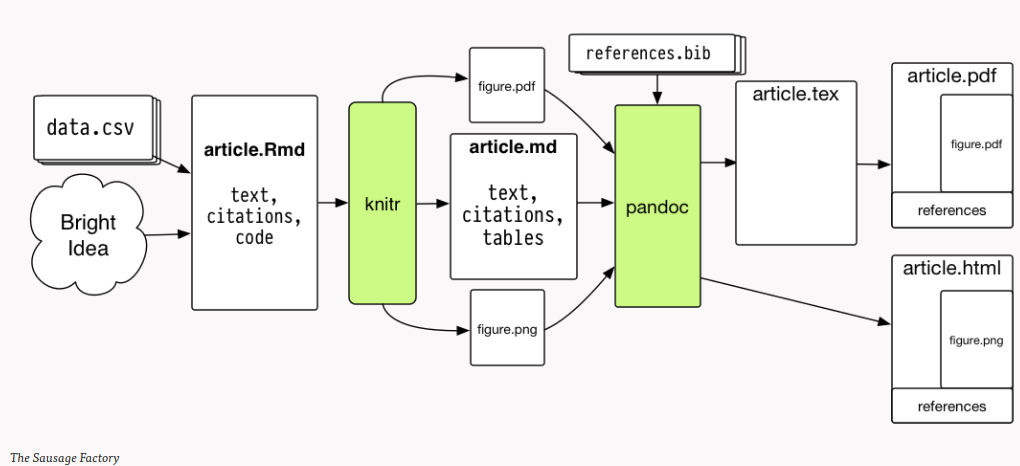
\includegraphics{images/healeysworkflow.png}

El documento central de trabajo es uno en formato .Rmd (Rmarkdown), que combina texto en Markdown y código R, lo que se detalla más abajo. La librería \texttt{Knitr} hace la transformación de este documento a formatos como html y/o pdf, para lo cual utiliza el convertidor pandoc.

No es necesario conocer al detalle todos los elementos de este flujo para hacer funcionar un documento dinámico, sino básicamente dos: 1) Markdown, y 2) Trozos de código. Vamos por parte.

\hypertarget{trozos-chunks-de-cuxf3digo}{%
\subsubsection{Trozos (chunks) de código}\label{trozos-chunks-de-cuxf3digo}}

La caracteristica principal de \texttt{Knitr} es que identifica las secciones de código en la hoja y los ejecuta mediante R. Estos trozos de código se encuentran delimitados de la siguiente manera:

\begin{verbatim}
```{r}
    4+5
```
\end{verbatim}

Es decir, todo lo que comience por \texttt{\textasciigrave{}\textasciigrave{}\textasciigrave{}r} y termine con \texttt{\textasciigrave{}\textasciigrave{}\textasciigrave{}} será identificado como código de análisis (el atajo para generar un chunk en RStudio es \texttt{ctrl+alt+i})

\hypertarget{tipos-de-chunks}{%
\subsubsection{Tipos de chunks}\label{tipos-de-chunks}}

En general hay cinco opciones básicas de edición relacionadas con chunks y su visualización en el documento final. Esto se maneja mediante opciones que aparecen al inicio en el chunk, luego de la letra \texttt{r}

\begin{enumerate}
\def\labelenumi{\arabic{enumi}.}
\tightlist
\item
  código y resultado (opción por defecto)
\end{enumerate}

\begin{verbatim}
```{r}
1 + 1
```
\end{verbatim}

Resulta

\begin{Shaded}
\begin{Highlighting}[]
\DecValTok{1} \OperatorTok{+}\StringTok{ }\DecValTok{1}
\end{Highlighting}
\end{Shaded}

\begin{verbatim}
## [1] 2
\end{verbatim}

\begin{enumerate}
\def\labelenumi{\arabic{enumi}.}
\setcounter{enumi}{1}
\tightlist
\item
  solo código, ocultando resultados:
\end{enumerate}

\begin{verbatim}
```{r, results='hide'}
1 + 1
```
\end{verbatim}

Resulta:

\begin{Shaded}
\begin{Highlighting}[]
\DecValTok{1} \OperatorTok{+}\StringTok{ }\DecValTok{1}
\end{Highlighting}
\end{Shaded}

\begin{enumerate}
\def\labelenumi{\arabic{enumi}.}
\setcounter{enumi}{2}
\tightlist
\item
  solo resultado
\end{enumerate}

\begin{verbatim}
```{r, echo=FALSE}
1 + 1
```
\end{verbatim}

Resulta:

\begin{verbatim}
## [1] 2
\end{verbatim}

\begin{enumerate}
\def\labelenumi{\arabic{enumi}.}
\setcounter{enumi}{3}
\tightlist
\item
  ni código ni resultado \texttt{\{r\ echo=FALSE\ results=\textquotesingle{}hide\textquotesingle{}\}}
\item
  resultado ``tal cual como es'': \texttt{\{r\ results=\textquotesingle{}asis\textquotesingle{}\}} se utiliza principalmente para comandos de generación de tablas, que arrojan un código que luego puede ser interpretado por otro lenguaje (por ejemplo, html)
\end{enumerate}

\hypertarget{trabajando-con-documentos-dinuxe1micos-en-rstudio}{%
\subsection{Trabajando con documentos dinámicos en RStudio}\label{trabajando-con-documentos-dinuxe1micos-en-rstudio}}

RStudio es principalmente un editor para análisis de datos con R, pero últimamente ha ido incorporando herramientas para reportes dinámicos. Para ello utiliza un tipo de archivos con extensión \texttt{Rmd} que significa Rmarkdown. Y en este contexto Rmarkdown es la forma en que Rstudio identifica los archivos que combinan texto y código.

Para generar un archivo Rmarkdown, simplemente new file \textgreater{} Rmarkdown

\includegraphics{images/rmarkdown.gif}

Y luego para convertir este documento, presionar el boton \texttt{Knitr}.

El generador de documentos por defecto trae un texto de ejemplo donde hay analisis y tablas, y además dos cosas:

\begin{itemize}
\item
  \textbf{Preámbulo o YAML (Yet Another Markdown Language)}: esta sección del inicio que se encuentra enmarcada entre \texttt{-\/-\/-} incluye algunos datos básicos del documento que luego se consideran al momento de convertirlo al documento editado final. Por ejemplo, si se prefiere que la conversión sea a html, se incluye la opción \texttt{output:\ html\_document}

\begin{verbatim}
---
title: "nuevo"
author: "jc"
date: "5/30/2019"
output: html_document
---
\end{verbatim}
\item
  \textbf{Chunk de opciones generales}: va al inicio del documento, luego del YAML. En general, la que aparece por defecto \texttt{echo=TRUE} se refiere a que se muestren los resultados de los chunks de código.
\end{itemize}

\hypertarget{reproducibilidad-1}{%
\section{Reproducibilidad}\label{reproducibilidad-1}}

\bibliography{book.bib,packages.bib,openscience.bib}


\end{document}
